\index{Generate Model}
\index{Modeling!Generate}

In order to be able to generate \gdcases{} and categories from a model, you must have:
\begin{itemize}
\item Created a modeling \gdproject{} \bxpref{TasksMBTCreateProject}.
\item Created \bxpref{TasksMBTCreateModel} or imported \bxpref{TasksMBTImport} a model diagram.
\item Created \bxpref{newproject} or opened \bxpref{loadproject} a \app{} \gdproject{}. 
\end{itemize}

\begin{enumerate}
\item When you are ready to generate, select:\\
\bxmenu{Modeling}{Generate}{}\\ from the menu or select the \bxcaption{Generate} button on the toolbar \gdmarpar{../../../share/PS/transform}{Generate}.
\item In the dialog that appears (\bxfigref{GenerateDialog}), you can configure what you want to generate. 

\begin{figure}[h]
\begin{center}
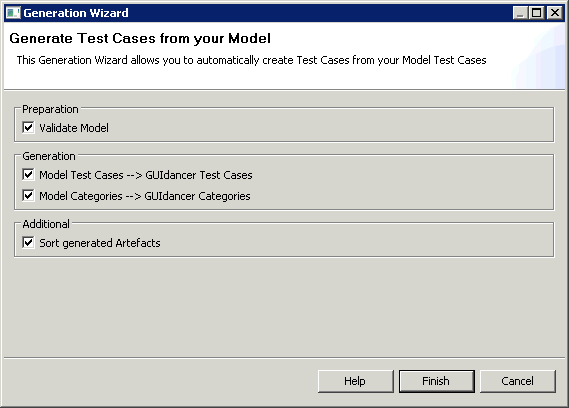
\includegraphics{Tasks/Modelling/PS/GenerateDialog}
\caption{Generation Dialog}
\label{GenerateDialog}
\end{center}
\end{figure} 


\begin{description}
\item [Validating]{ the model is the prerequisite for all other options. It ensures that the model can be successfully generated.} 
\item [Model \gdcases{} to \app{} \gdcases{}:]{This converts any \gdcases{} you have created in the model to corresponding \app{} \gdcases{} in the \gdtestcasebrowser{}. Generated \gdcases{} have a green corner. }
\item [Model categories to \app{} categories:]{This converts categories you have created in the model to categories in the \gdtestcasebrowser{}. Generated categories are slightly green. }
\item [Sort generated artefacts:]{This option organizes your \gdcases{} into categories as specified in the model. If you turn this option off, your \gdcases{} will not be created in the modeled categories, nor will any \gdcases{} from previous generations be moved back into the modeled categories in the \gdtestcasebrowser{} (if you re-organized \gdcases{} for example).}
\end{description}
\item Click \bxcaption{Finish} to start the generation. During the generation, the status of the various actions is shown in the console. Once the generation is complete, you will be able to see the items you generated in the \gdtestcasebrowser{}. 
\bxtipp{Parameters that are part of generated \gdcases{} are \bxname{locked} by default, and cannot be changed or deleted. You can see the parameters and unlock them in the \gdtestcaseeditor{} using the \bxname{edit parameters} dialog \bxpref{editparams}. }
\item Once the \gdcases{} have been generated, you can fill them with the necessary \gdcases{} from the library in \app{} to create your tests. 
%regeneration, model always right
\end{enumerate}

\subsubsection{Regenerating models}
After generating a model for the first time, you may want to make changes and regenerate it. This is not a problem in \app{} -- it will not result in duplicates of previously created items being made. Any changes made to the model (if you have added or renamed items, for example) will be reflected in the \gdcase{} generation. However, there are two points to bear in mind:

\begin{description}
\item [Deleting objects from the model:]{Any objects you delete from the model will not be deleted from the \gdcase{} browser. }
\item [The model takes precedence over other changes:]{If you have made changes to the generated \gdcases{} in the \gdtestcasebrowser{} or \gdtestcaseeditor{} (e.g. renamed them, added other \gdcases{}), these changes will be lost when you regenerate the model. }
\end{description}
